\label{chap:machine_learning}

In questa tesi considereremo il Machine Learning come il processo che consente
la creazione di modelli in grado di apprendere autonomamente dai dati. Un
modello è costituito da un insieme di parametri e una struttura che elabora i
dati di input per produrre un output. I parametri vengono appresi durante la
fase di addestramento, in cui il modello esamina vari esempi e regola i propri
parametri di conseguenza. Gli iperparametri, d'altra parte, sono valori
definiti dall'utente prima dell'inizio dell'addestramento che influenzano la
struttura del modello e il suo comportamento durante l'addestramento.

Prima di esplorare i modelli specifici, ci concentreremo sul processo di
creazione dei modelli di Machine Learning, e vedremo come l'automatizzazione
di questo processo, attraverso l'impiego di una \textbf{pipeline}, possa
ottimizzarne l'efficienza e l'efficacia.

Il processo di creazione di un modello di Machine Learning si compone di vari
passaggi: l'estrazione dei dati, la loro preparazione e l'addestramento del
modello. Una pipeline collega questi passaggi in sequenza,
incapsulandoli in un'entità che, dall'esterno, può essere utilizzata come se
fosse il modello stesso. Questa pipeline può essere rappresentata come un
Grafo Aciclico Diretto (DAG), dove i dati fluiscono in una sola direzione,
evitando cicli, e dove ogni nodo in questo grafo rappresenta una fase distinta
del processo (vedi figura~\ref{fig:ml_pipeline_dag}).

\begin{figure}[!ht]
    \centering
    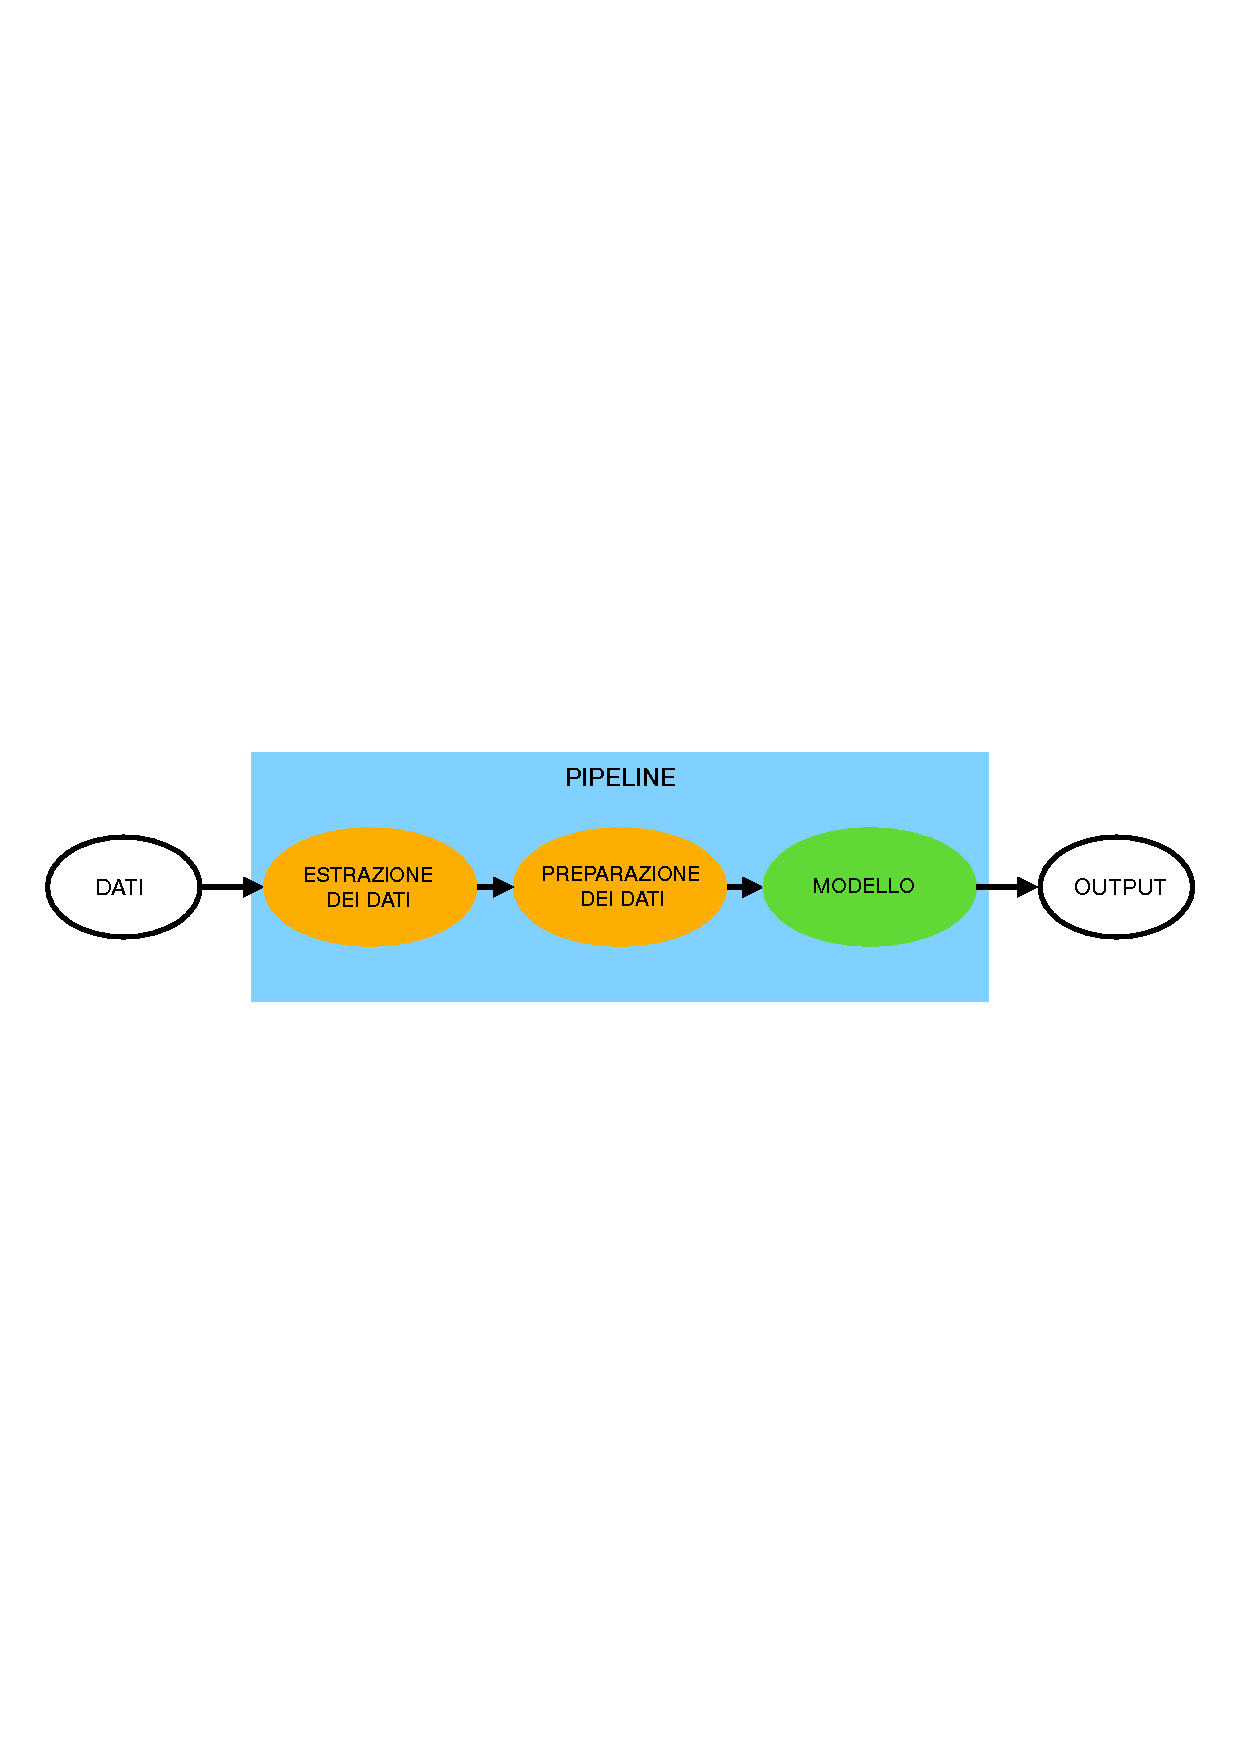
\includegraphics[trim=0 12.5cm 0 12.5cm, clip, width=\linewidth]{pipeline}
    \caption{Rappresentazione di una pipeline di Machine Learning come un
    grafo orientato senza cicli}
    \label{fig:ml_pipeline_dag}
\end{figure}

L'uso di una pipeline nel Machine Learning ci permette di ottenere i seguenti
vantaggi:
\begin{itemize}
    \item[\textit{Efficacia}] \textbf{Estensione della ricerca degli iperparametri ad altri
        componenti}: Mentre l'individuazione dei parametri migliori per un
        modello avviene in modo automatico durante l'addestramento, la ricerca
        degli iperparametri migliori richiede sperimentazioni multiple,
        testando diversi valori e valutando i risultati del modello secondo
        metriche prestabilite. Dato che esternamente una pipeline funziona
        esattamente come un modello, è possibile estendere la ricerca degli
        iperparametri migliori a componenti non direttamente correlati al
        modello stesso, come quelle legate all'estrazione e alla preparazione
        dei dati. Poiché anche la ricerca degli iperparametri è
        automatizzabile, è possibile testare automaticamente diverse tecniche
        di preparazione dei dati, semplicemente integrando il componente alla
        pipeline.
    \item [\textit{Efficienza}]\textbf{Sperimentazione rapida}: L'organizzazione di tutti i
        passaggi in una pipeline può accelerare notevolmente la
        sperimentazione. Questo è particolarmente utile quando si prevede di
        testare vari iperparametri o di utilizzare differenti sottoinsiemi di
        dati. Infatti, incapsulando le operazioni delle diverse componenti in
        un unico elemento che le esegue sequenzialmente, si evita di ripetere
        le stesse operazioni più volte, risultando in un risparmio di tempo
        significativo.
\end{itemize}

Nelle sezioni seguenti, descriveremo come sono stati affrontati i vari
passaggi nella creazione di un modello di Machine Learning per
l'identificazione dei job zombie e come si è cercato di integrare ciascun
componente alla pipeline.

\section{Estrazione dei dati}

Procediamo con l'estrazione di un dataset tramite una query SQL che interroga
le tabelle \texttt{hj} e \texttt{htjob}, selezionando i dati rilevanti.
Ricordando che:
\begin{itemize}
    \item La tabella \texttt{hj} contiene lo stato dei job, rappresentato da
        serie storiche di misurazioni (come \texttt{runtime}, \texttt{ram},
        \texttt{swap}, \texttt{disk}, ecc.),
        durante la loro esecuzione.
    \item La tabella \texttt{htjob} fornisce informazioni sull'esito dei job,
        indicando se sono falliti o meno.
\end{itemize}

% fail 
% jobid.idx.submitnode
%jobid e idx sono creati dal Submit Node al "concepimento" del job (es.
%'sn-01', 'ce03-htc', ...). I S.N. sono indipendenti tra loro per cui in linea
%di principio possono esistere due job diversi con (jobid,idx) uguale (in tal
%caso vengono da S.N. diversi)

%Ci sono due momenti diversi: il batch system puo' terminare LUI un job anche
%se non ha alcun problema (per una serie di ragioni) e quella info e' in
%jobstatus, Poi c'e' lo exitstatus dell'eseguibile vero e proprio: di questo
%sappiamo che se e' 0 allora e' ok, se e' != 0 e' uscito con errore (quale sia
%lo sa il suo owner).

La query esegue le seguenti operazioni:
\begin{itemize}
    \item Seleziona i job che hanno iniziato e finito la loro esecuzione nel
        periodo temporale specificato.
    \item Esegue un JOIN delle tabelle utilizzando l'identificativo univoco di
        ciascun job (\textit{jobid.idx\_submitnode}) e il timestamp. Questo
        timestamp sfrutta l'indice presente nella tabella
        \texttt{hj} per gestire in maniera efficiente le grandi dimensioni di
        questa tabella\footnote{La logica dietro questo consiste
            nel selezionare un job da \texttt{htjob} e successivamente
            cercarlo in \texttt{hj} limitando la ricerca ai record che
            rientrano nel periodo in cui \texttt{hj.ts} è compreso tra
            \texttt{htjob.starttimeepoch} e \texttt{htjob.eventtimeepoch}.
            Questo permette di restringere notevolmente la ricerca nella
            tabella \texttt{hj} per ogni job selezionato da \texttt{htjob} ed
        evitare di scansionare l'intera tabella.}. Poiché la tabella \texttt{hj} contiene più record per
        ogni job, la query li raggruppa per job. In seguito, mediante l'uso
        dell'operatore \verb|ARRAY_AGG|, le serie storiche vengono trasformate
        in liste di valori.
    \item Filtra i job con un tempo di esecuzione superiore a un'ora
        (\verb|runtime > 3600|), in quanto i job più brevi sono considerati
        irrilevanti per lo scopo dello studio.
\end{itemize}

Il risultato di questa query è un dataset come mostrato nella
figura~\ref{fig:dataset_from_join_hj_htjob}, dove ogni riga rappresenta un job
e le colonne includono: 

\begin{itemize}
    \item \texttt{job}: identificativo univoco per ogni job.
    \item \texttt{queue}: gruppo di appartenenza dell'utente che ha sottomesso
        il job.
    \item \texttt{fail}: una variabile booleana che indica se il job è fallito.
    \item \texttt{mint} e \texttt{maxt}: il tempo minimo e massimo di
        esecuzione del job.
    \item \texttt{t}, \texttt{ram}, \texttt{swap}, \texttt{disk}: liste di
        valori che rappresentano le serie storiche di misurazioni.
\end{itemize}

\begin{figure}[!ht]
    \centering
    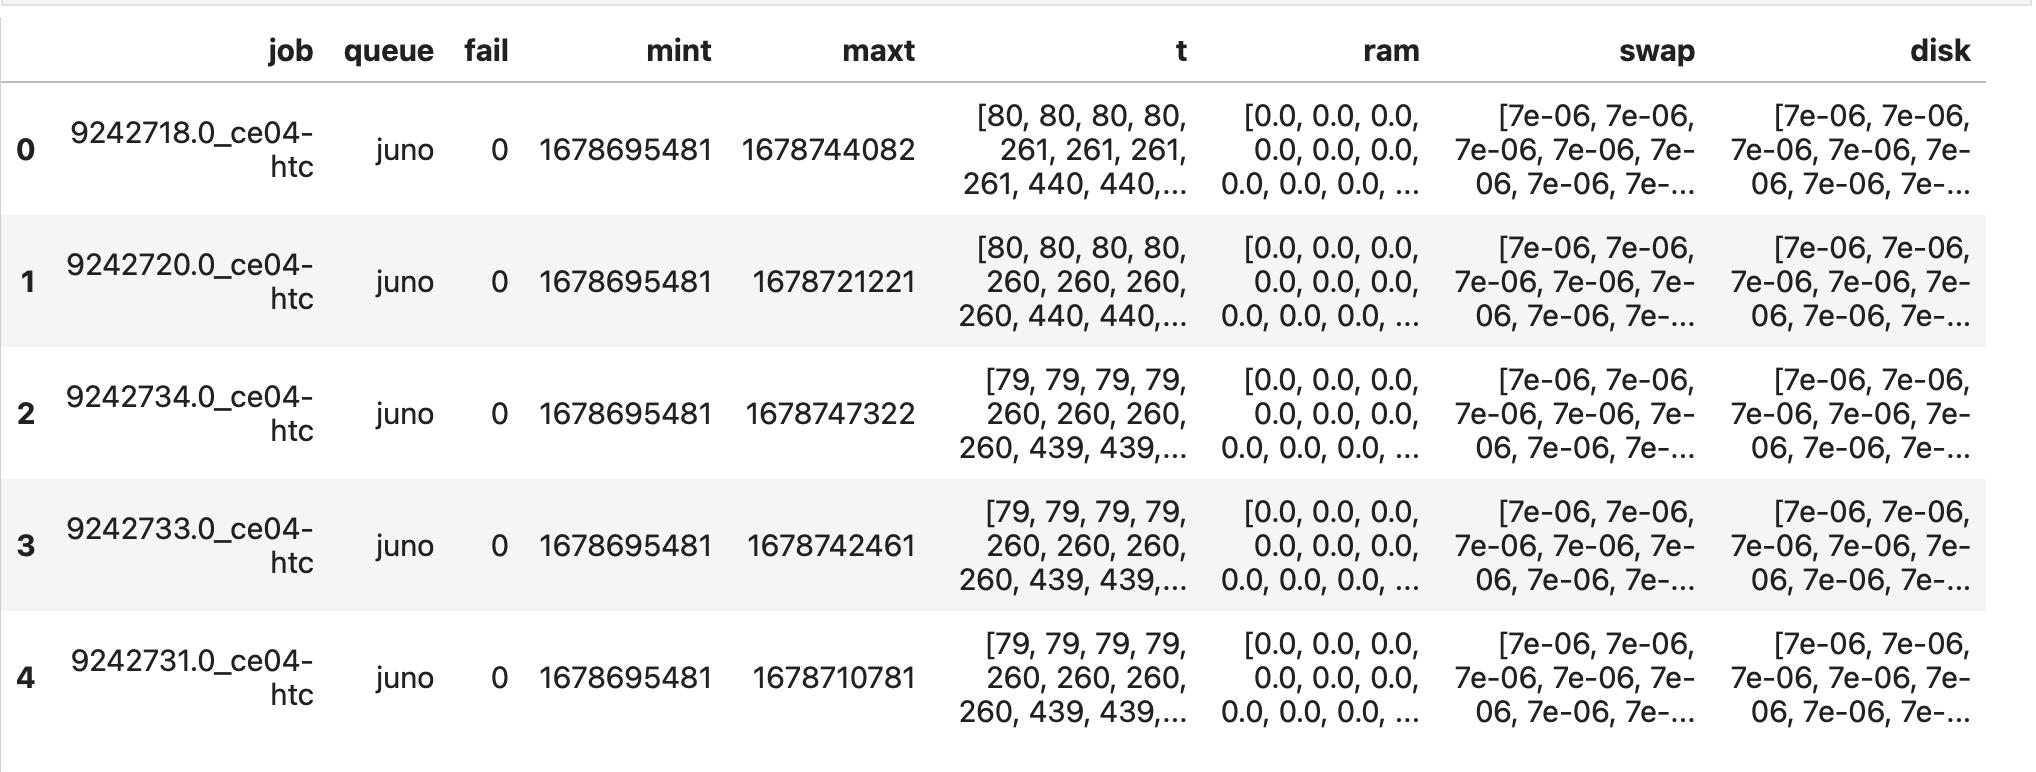
\includegraphics[width=0.95\textwidth]{dataset}
    \caption{Le prime cinque righe del dataset}
    \label{fig:dataset_from_join_hj_htjob}
\end{figure}

Tuttavia, il dataset estratto non è ancora pronto per l'addestramento del
modello e necessita di ulteriori trasformazioni da parte del componente
successivo. Questo passaggio non è stata integrato nella pipeline, in quanto,
nell'ambiente operativo reale, si prevede che questa lavori direttamente con i
dati forniti da HTCondor, eliminando così la necessità di estrarre dati da un
database SQL.

\section{Preparazione dei dati}

La preparazione dei dati è essenziale nel Machine Learning. Prima di tutto, è
necessario convertire i dati in numeri, dato che gli algoritmi di Machine
Learning lavorano esclusivamente con dati in tale forma. Inoltre, la qualità e
la quantità dei dati sono determinanti per l'efficacia del modello. Se i dati
disponibili sono insufficienti o di bassa qualità, i risultati saranno
scadenti a prescindere dalla complessità del modello utilizzato. Tipicamente,
maggiore è la complessità di un modello, tanto più esso richiederà una grande
quantità di dati di alta qualità.

Per realizzare ciò, è stata creata una classe denominata
\texttt{Preprocessor}, che riceve in input un dataset e restituisce in output
un dataset modificato, eseguendo una serie di operazioni intermedie. Queste
operazioni possono essere ricondotte a tre categorie: l'aggiunta, la rimozione
e la trasformazione di colonne. Le operazioni effettuate sono configurabili
attraverso parametri definiti nel costruttore della classe al momento della
sua istanziazione. Quando questo componente viene inserito all'interno di una
pipeline, tali parametri fungono da iperparametri, permettendo di esplorare
diverse configurazioni per identificare quale produca i risultati migliori.

% immagine

In aggiunta, questa classe è stata implementata seguendo il design pattern
Template Method, nel quale i passaggi di un algoritmo vengono divisi in metodi
separati, e successivamente invocati da un metodo denominato template (vedi
figura~\ref{fig:uml_preprocessor}). La superclasse definisce lo scheletro
dell'algoritmo, consentendo alle sottoclassi di personalizzare alcuni passaggi
sovrascrivendo alcuni metodi. In questo modo, è possibile codificare la parte
invariante dell'algoritmo una sola volta nella superclasse, lasciando alle
sottoclassi il compito di implementare i comportamenti che possono variare. In
pratica, l'uso di questo pattern in questa classe ci consente di aggiungere,
modificare e rimuovere passaggi dall'algoritmo in modo semplice ed immediato,
senza la necessità di dover intervenire sul codice della classe principale.

\begin{figure}[!ht]
   \centering
   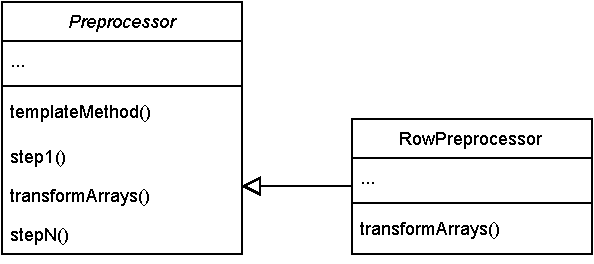
\includegraphics[width=0.5\linewidth]{preprocessor}
   \caption{Diagramma UML della classe \texttt{Preprocessor}, illustrante
   l'implementazione del design pattern Template Method}
   \label{fig:uml_preprocessor}
\end{figure}

Dopo aver delineato la struttura generale della classe \texttt{Preprocessor},
descriveremo ora le trasformazioni effettuate dal metodo
\texttt{preprocess()}, che funge da metodo template, nella preparazione dei
dati.

\subsection{Preparazione delle serie storiche}

Nella sezione~\ref{sec:job_analysis}, abbiamo identificato alcuni problemi
nelle misurazioni registrate da HTCondor relative allo stato dei job. Un
problema è la presenza di valori ripetuti all'interno delle serie storiche.
Queste serie sono attualmente rappresentate come liste di valori, che non
corrispondono al formato numerico richiesto dai modelli di Machine Learning.
Pertanto, è necessario non solo rimuovere le ripetizioni, ma anche convertire
queste serie storiche in un formato di dati strutturato.

\paragraph{Sottocampionamento.} Applicando un'operazione di
convoluzione\footnote{Operazione matematica che consiste nell'applicare un
    filtro di dimensione finita lungo la sequenza di valori. Il filtro, di
    solito di piccole dimensioni, viene fatto scorrere su tutta la sequenza, e
    in ogni posizione si calcola una somma pesata tra i valori della sequenza
    e quelli del filtro. Questo processo trasforma la sequenza originale in
    una nuova attraverso la formula: $$(S\ast
    K)(i)=\displaystyle\sum_{m=-d}^{d}S(m)\cdot K(i-m)$$ dove $S$ è la
sequenza originale, $K$ è il filtro e $d$ è l'intero inferiore della metà
della lunghezza del filtro.} con un passo (\textit{stride}) di 5 e un filtro
con elementi $\frac{1}{5}$, possiamo effettuare un sottocampionamento della
sequenza originale. Ciò comporta di ottenere una nuova sequenza, la cui
lunghezza è pari a un quinto della lunghezza della serie storica originale. In
pratica, il filtro calcola la media di ogni gruppo di cinque valori
consecutivi. Se questi cinque valori sono identici, il risultato sarà il
valore stesso, che sostituisce la sequenza dei cinque valori, eliminando le
ripetizioni nella nuova sequenza.

\paragraph{Trasformazione delle multiple serie storiche multivariate.} Sebbene
durante il processo di estrazione dei dati le serie storiche multivariate
siano state rappresentate come liste, il dataset rappresenta ancora le tre
dimensioni delle multiple serie multivariate: job (righe), variabili (colonne)
e time step (liste), come illustrato nella
figura~\ref{fig:multiple_multivariate_time-series}. Una possibile soluzione
potrebbe essere quella di trasformare le liste in una singola statistica, come
la media o il massimo, ma ciò cancellerebbe qualsiasi indicazione
sull'evoluzione temporale di ciascun job. Il nostro obiettivo è quello di
introdurre nuove feature che possano riflettere la tridimensionalità originale
dei dati. Tuttavia, prima di procedere, è necessario assicurarsi che tutte le
serie storiche siano uniformate alla stessa lunghezza.

\begin{figure}[!ht]
   \centering
   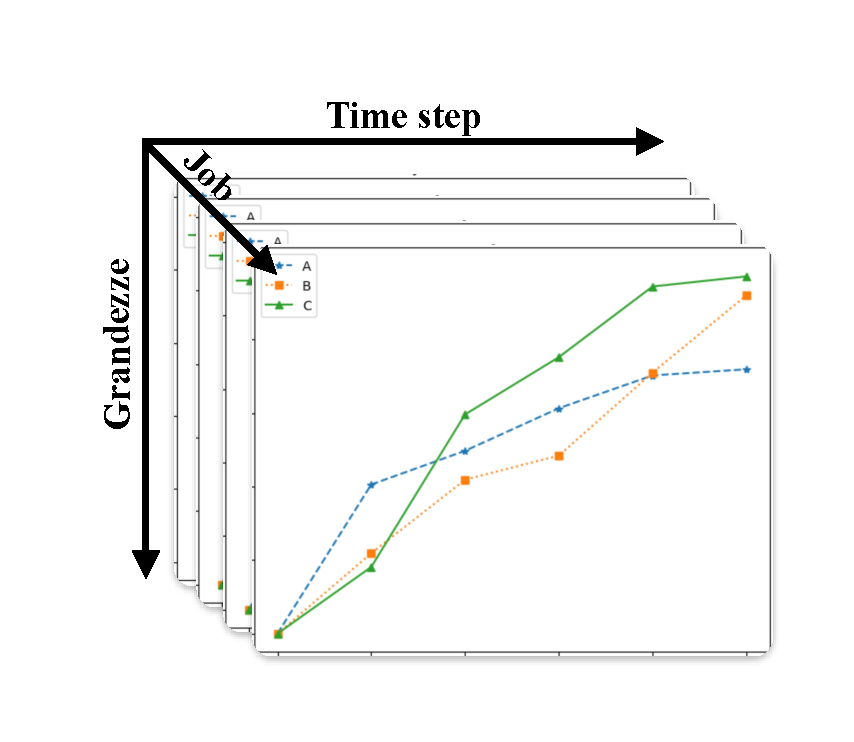
\includegraphics[trim=0cm 1.5cm 0cm 1.5cm, clip, width=0.5\linewidth]{multiple_multivariate_time-series}
   \caption{Rappresentazione tridimensionale delle multiple serie storiche
   multivariate}
   \label{fig:multiple_multivariate_time-series}
\end{figure}

Per gestire serie di dati con lunghezze diverse, possiamo utilizzare due
strategie: lo zero-padding e il troncamento. Lo zero-padding si applica alle
sequenze più corte, aggiungendo zeri fino a raggiungere una lunghezza
prefissata. Invece, il troncamento si usa per ridurre le sequenze più lunghe,
tagliandole fino a che non raggiungono la stessa lunghezza prestabilita. La
classe \texttt{Preprocessor} implementa entrambe le tecniche: stabilisce una
lunghezza fissa per tutte le sequenze, troncando quelle che eccedono questa
lunghezza e applicando lo zero-padding a quelle che non la raggiungono.

Una volta ottenute serie storiche di uguale lunghezza, vengono applicate le
seguenti trasformazioni, in base al modello utilizzato:

\begin{itemize}
    \item \textbf{Trasformazione in colonne}: Ogni elemento di ogni lista diventa una colonna
        separata nel dataset. Ad esempio, con un sottocampionamento a 15
        minuti per un giorno, avremo 96 time step, corrispondenti a 96 colonne
        per ciascuna serie temporale.
    \item \textbf{Trasformazione in righe}: 
        Gli elementi nelle stesse posizioni nelle liste formano righe
        distinte. Quindi, con un sottocampionamento a 15 minuti per un giorno,
        otteniamo 96 righe per ogni job.
\end{itemize}

\subsection{Creazione delle feature} % ESTIMATE 2h

% dopo la trasformazione abbiamo tutte le colonne delle serie storiche in
% formato numerico, ma alcune colonne non sono ancora nel formato richiesto.

\begin{figure}[!ht]
    \centering
    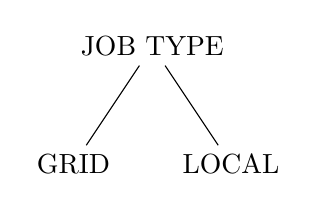
\begin{tikzpicture}[sibling distance=2cm]
        \node {JOB TYPE}
            child {node {GRID}}
            child {node {LOCAL}};
    \end{tikzpicture}
    \hspace{2cm}
    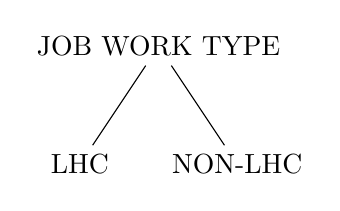
\begin{tikzpicture}[sibling distance=2cm]
        \node {JOB WORK TYPE}
        child {node {LHC}}
        child {node {NON-LHC}};
    \end{tikzpicture}
\end{figure}

%Complex nonlinear relationships may be teased out of the data.
% r how to best expose the underlying structure of the problem to the learning algorithms. This is the guiding light.
% non contiene dati duplicati e missing values

% your system will only be capable of learning if the training data enough
% relevant and not too many irrilevant ones. A critical part of the success of
% a machine learning project is coming up with a good set of features to train
% on.
% This process, called feature engineering

% molte colonne presenti nel dataset sono colonne derivanti dalle tabelle hj e
% htjob con colonne categoriche

% jobid e idx

% jobid e idx sono creati dal Submit Node al "concepimento" del job (es.
% 'sn-01', 'ce03-htc', ...). I S.N. sono indipendenti tra loro per cui in linea
% di principio possono esistere due job diversi con (jobid,idx) uguale (in tal
% caso vengono da S.N. diversi)%

% job work type

% job type

% one hot encoding 

% non verranno considerati i jobs con runtime <
% 1h, poichè non rilevanti per il sistema.

% variabili categoriche
% queue
% one hot encoding

\subsection{Etichettatura dei dati} % ESTIMATE 1h

% perché etichettare i dati

% Una possibile strategia:
% - usando htjob si trovano i job eliminati per "toomuchtime": sono quelli con
%   jobstatus = 3 e runtime ~=7gg (non c'è valore esatto!)
% - a questo punto possiamo possiamo impostare un supervised learning
%   guardando su hj come hanno "vissuto" quei job.

\subsection{Tecniche di bilanciamento dei dati} % ESTIMATE 5h

% undersample

% oversample

% class weighting in loss function

% Metriche

\section{Selezioni dei modelli}
\subsection{Modelli supervisionati}        
%L'input è rappresentato da un tensore 3D (batch size, time steps,
%features)
%To train the LSTM you use the typical Mini-batch training. Make sure
%you don't propagate the state for batch sample 𝑖 to sample 𝑖+1 in
%order to treat them individually (in Keras you set the stateful flag
%to False)
% Essentially, the author is describing a means for forecasting sales
% with LSTM whereby the model is trained on a mini-batch (or subset) of
% one series, and then a new series is selected.

%This would have the advantage of essentially creating a unified series
%that takes the characteristics of all weather stations into account -
%which allows for maximum utilisation of the data, as well as allowing
%the network to learn patterns from all stations - not just one or a
%select few.
%An RNN (or a Transformer) could use any of/all of the history that you
%give it. But that's assuming that the history is useful for the
%predictions you're making.
\subsection{Modelli non supervisionati}
